% WildfireIQ Kamloops -- Project Report
% Compiles with pdflatex (standard packages only).
\documentclass[11pt]{article}

\usepackage[T1]{fontenc}
\usepackage[utf8]{inputenc}
\usepackage{lmodern}
\usepackage[margin=1in]{geometry}
\usepackage{xcolor}
\usepackage{graphicx}
\usepackage{booktabs}
\usepackage{array}
\usepackage{titlesec}
\usepackage{enumitem}
\usepackage{tikz}
\usepackage{fancyhdr}
\usepackage[hidelinks]{hyperref}

\usetikzlibrary{positioning, arrows.meta}

% ==== Colour scheme (professional slate + ember accent)
\definecolor{ink}{HTML}{1F2A37}      % headings
\definecolor{ember}{HTML}{C2410C}    % accent
\definecolor{slate}{HTML}{475569}    % secondary text
\definecolor{mist}{HTML}{EEF2F6}     % light fills
\definecolor{line}{HTML}{CBD5E1}     % rules

\hypersetup{
  colorlinks=true,
  linkcolor=ember,
  urlcolor=ember,
}

% ==== Section styling
\titleformat{\section}{\color{ink}\Large\bfseries}{\thesection}{0.6em}{}
\titleformat{\subsection}{\color{ink}\large\bfseries}{\thesubsection}{0.6em}{}
\titlespacing*{\section}{0pt}{1.4em}{0.6em}

% ==== Header / footer
\pagestyle{fancy}
\fancyhf{}
\renewcommand{\headrulewidth}{0.4pt}
\renewcommand{\headrule}{\hbox to\headwidth{\color{line}\leaders\hrule height \headrulewidth\hfill}}
\fancyhead[L]{\small\color{slate}WildfireIQ Kamloops}
\fancyhead[R]{\small\color{slate}Project Report}
\fancyfoot[C]{\small\color{slate}\thepage}

% ==== Table helpers
\newcolumntype{L}[1]{>{\raggedright\arraybackslash}p{#1}}
\renewcommand{\arraystretch}{1.25}

% ==== A simple coloured callout box
\newcommand{\callout}[1]{%
  \par\medskip\noindent
  \colorbox{mist}{\parbox{\dimexpr\linewidth-2\fboxsep}{\color{ink}\small #1}}%
  \par\medskip}

\begin{document}

% ============================ COVER ============================
\begin{titlepage}
\thispagestyle{empty}
\color{ink}
\vspace*{1.2cm}

{\noindent\color{ember}\rule{\linewidth}{2.5pt}}
\vspace{0.8cm}

\noindent{\Huge\bfseries WildfireIQ Kamloops}\\[0.5cm]
{\noindent\LARGE A wildfire risk, air quality, and community preparedness platform for the Thompson-Okanagan}\\[0.6cm]

{\noindent\large\color{slate} Project Report and Final Implementation}

\vspace{0.6cm}
{\noindent\color{ember}\rule{\linewidth}{1pt}}

\vspace{2.2cm}
\noindent
\begin{tabular}{@{}ll@{}}
{\bfseries Author} & Deeparsh Singh Dang \\[0.3em]
{\bfseries Funding} & TRU Sustainability Research Grant, 2025--2026 \\[0.3em]
{\bfseries Region} & Thompson-Okanagan, British Columbia \\[0.3em]
{\bfseries Licence} & MIT (code), CC-BY-4.0 (written content) \\
\end{tabular}

\vfill
\callout{\textbf{Informational only.} This platform supports public awareness and planning. It does not replace official guidance from the BC Wildfire Service, BC Emergency Management Climate Readiness, or Environment and Climate Change Canada.}

\noindent{\color{slate}\small Generated for project handoff.}
\end{titlepage}

% ============================ TOC ============================
\newpage
\tableofcontents
\newpage

% ============================ 1. OVERVIEW ============================
\section{Project Overview}

WildfireIQ Kamloops is a web platform that brings wildfire information into one
place for people who live in the Thompson-Okanagan region of British Columbia.
It answers four everyday questions: where are the fires right now, is the air
safe to breathe, how do I get my home and family ready, and how has fire risk
changed over time.

The platform is built around a three-dimensional globe of British Columbia.
Live data layers sit on top of the globe, and three supporting pages cover air
quality, household preparedness, and long-term climate trends. Two machine
learning models add a forward-looking view: one estimates daily wildfire risk,
the other forecasts air quality for the next two days.

Everything runs on free and open data sources, stores no personal information,
and is released as open source. The goal was a tool that is genuinely useful to
a resident, a journalist, or a local official, and that is honest about what it
can and cannot tell you.

\callout{\textbf{At a glance.} 4 connected modules, 17 automated data jobs, 32
API endpoints, 2 validated machine learning models, and 23 years of historical
fire and weather records, all served locally at no cloud cost.}

% ============================ 2. WHAT IT DOES ============================
\section{What the Platform Does}

The platform has four parts. Each one is described below in plain terms.

\begin{table}[h]
\centering
\small
\begin{tabular}{@{}L{3.1cm}L{10.5cm}@{}}
\toprule
\textbf{Module} & \textbf{What it shows} \\
\midrule
\textbf{3D Globe} &
The home screen. Shows active fires, satellite heat detections, evacuation
zones, fire-weather stations, a smoke forecast you can step through hour by
hour, and an AI risk map. Layers can be turned on and off, and each one has a
plain-language explanation. \\
\textbf{Air Quality} &
A live air quality reading for Kamloops, a forecast for the next 48 hours with
an honest uncertainty range, a six-pollutant breakdown, a one-year smoke
calendar, and health guidance from Health Canada. \\
\textbf{Preparedness Hub} &
A personalised FireSmart checklist that adapts to your home type and season, a
live check of whether your neighbourhood is under an evacuation order, progress
badges, and a private share link. Nothing leaves your device. \\
\textbf{Climate Trends} &
A scrolling story of how the region's fire seasons have changed over 27 years,
with clear trend lines, and a look ahead under different emission scenarios. \\
\bottomrule
\end{tabular}
\caption{The four modules of WildfireIQ Kamloops.}
\end{table}

\subsection{Key numbers}

\begin{table}[h]
\centering
\small
\begin{tabular}{@{}L{6.5cm}L{6.5cm}@{}}
\toprule
\textbf{Item} & \textbf{Figure} \\
\midrule
Historical fire records (1999 to today) & 15,996 incidents \\
Daily weather history & 10,010 days (about 27 years) \\
Air quality stations shown (province-wide) & 34 \\
Fire-weather stations & 18 \\
AI risk map cells (Thompson-Okanagan) & 185 hexagons \\
FireSmart checklist actions & 30 \\
Smoke forecast steps & 73 hourly snapshots \\
Automated tests passing & 47 backend, 22 frontend \\
\bottomrule
\end{tabular}
\caption{Selected figures from the final build.}
\end{table}

% ============================ 3. DATA ============================
\section{Where the Data Comes From}

Every layer is built from a free, public data source. The platform downloads,
cleans, and stores the data, then serves it to the browser. No source requires
payment, and only three need a free sign-up key (Cesium for the globe, NASA for
satellite heat detections, and WAQI for pollutants).

\begin{table}[h]
\centering
\small
\begin{tabular}{@{}L{3.6cm}L{5.6cm}L{3.6cm}@{}}
\toprule
\textbf{Layer} & \textbf{Source} & \textbf{Coverage} \\
\midrule
Active fires & BC Wildfire Service (DataBC) & All of BC \\
Satellite heat detections & NASA FIRMS (VIIRS, MODIS) & All of BC \\
Evacuation zones & BC Emergency Management & All of BC \\
Fire Weather Index & Open-Meteo, computed in-house & 18 BC stations \\
Air quality (live) & Environment Canada GeoMet & All of BC \\
Air quality (history) & Open-Meteo CAMS & Kamloops \\
Smoke forecast & Environment Canada RAQDPS-FW & All of BC \\
Weather & Open-Meteo & Kamloops \\
Climate projections & ClimateData.ca structure & Regional \\
Globe terrain and imagery & Cesium Ion & Global \\
\bottomrule
\end{tabular}
\caption{Data sources and the area each layer covers.}
\end{table}

\subsection{How the data stays current}

Seventeen small jobs run on timers inside the application. Active fires refresh
every 15 minutes, evacuation zones every 5 minutes, weather and air quality
every hour, and the smoke forecast every six hours. When the app starts, it
checks each source and refreshes anything older than 30 minutes, so the screen
shows current information within seconds of opening rather than waiting for the
next scheduled update.

\callout{\textbf{Honest about freshness.} A satellite heat detection is a
``worth investigating'' signal, not a confirmed fire. A high Fire Weather Index
describes dangerous conditions, not an active fire. The platform spells this out
on every layer so readers are not misled.}

% ============================ 4. AI ============================
\section{How the AI Works}

Two machine learning models add a forward-looking view. Both were trained on
real historical records and tested on years the models had never seen, which is
what makes their accuracy figures trustworthy rather than memorised.

\subsection{Wildfire risk model}

This model estimates the chance that a fire starts somewhere in the region on a
given day, using the day's weather and fire-weather conditions. It learned from
23 years of records, was tuned on 2022, and was tested on a held-out 2023.

The model is a gradient-boosted decision tree (LightGBM). On the unseen 2023
test year it scored a precision-recall area of 0.66, clearly ahead of the
traditional fire-weather-threshold method at 0.52. The single regional estimate
is then scaled for each map hexagon by how often that specific area has burned
in the past.

\subsection{Air quality forecaster}

This model predicts fine-particle pollution (the harmful part of smoke) for the
next 48 hours. Instead of a single guess, it produces a low, middle, and high
estimate, so the chart can show an honest range that widens when the model is
less certain.

\begin{table}[h]
\centering
\small
\begin{tabular}{@{}L{4cm}r r@{}}
\toprule
\textbf{Forecast horizon} & \textbf{Model error} & \textbf{Simple baseline} \\
\midrule
6 hours  & 2.27 & 2.85 \\
12 hours & 3.20 & 4.06 \\
24 hours & 3.82 & 3.63 \\
48 hours & 3.32 & 3.92 \\
\bottomrule
\end{tabular}
\caption{Air quality forecast error in micrograms per cubic metre (lower is
better). The model beats the ``tomorrow equals today'' baseline at most
horizons.}
\end{table}

% ============================ 5. HOW IT IS BUILT ============================
\section{How It Is Built}

The platform has two halves: a browser front end that draws the globe and pages,
and a back end that collects data and runs the models. They talk over a simple
web interface.

\begin{figure}[h]
\centering
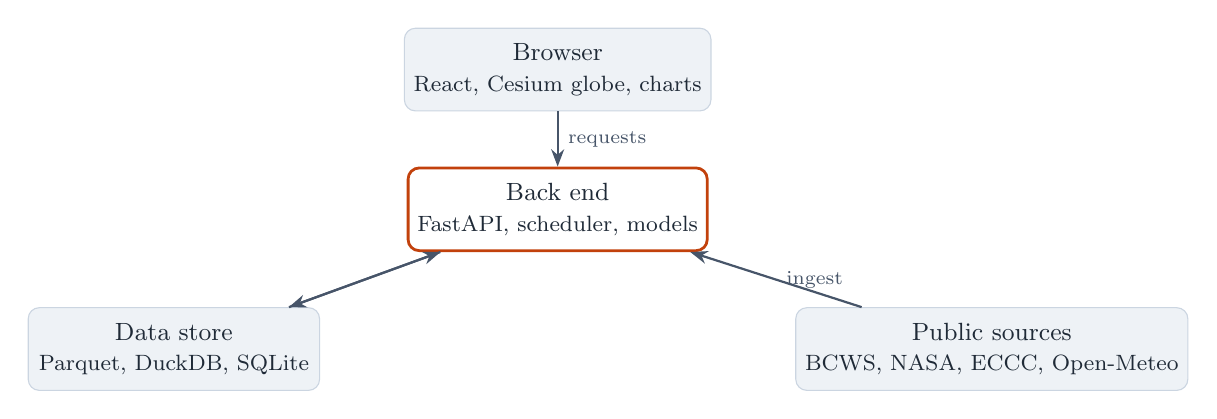
\begin{tikzpicture}[
  node distance=0.7cm and 1.1cm,
  box/.style={rectangle, rounded corners, draw=line, fill=mist, text=ink,
    align=center, minimum height=1.05cm, minimum width=3.7cm, font=\small},
  accent/.style={rectangle, rounded corners, draw=ember, line width=1pt,
    fill=white, text=ink, align=center, minimum height=1.05cm,
    minimum width=3.7cm, font=\small},
  arr/.style={-{Stealth[length=2.2mm]}, draw=slate, thick}
]
\node[box] (browser) {Browser\\\footnotesize React, Cesium globe, charts};
\node[accent, below=of browser] (api) {Back end\\\footnotesize FastAPI, scheduler, models};
\node[box, below left=of api] (data) {Data store\\\footnotesize Parquet, DuckDB, SQLite};
\node[box, below right=of api] (sources) {Public sources\\\footnotesize BCWS, NASA, ECCC, Open-Meteo};

\draw[arr] (browser) -- node[right, font=\scriptsize\color{slate}] {requests} (api);
\draw[arr] (api) -- (data);
\draw[arr] (sources) -- node[right, font=\scriptsize\color{slate}] {ingest} (api);
\draw[arr] (data) -- (api);
\end{tikzpicture}
\caption{High-level architecture. Public sources feed the back end on timers;
the browser reads cleaned data through the API.}
\end{figure}

\begin{table}[h]
\centering
\small
\begin{tabular}{@{}L{3cm}L{10.5cm}@{}}
\toprule
\textbf{Layer} & \textbf{Main tools} \\
\midrule
Front end & React, TypeScript, Vite, CesiumJS (3D globe), Tailwind, Visx (charts) \\
Back end & Python, FastAPI, APScheduler (timers), LightGBM (models) \\
Storage & Parquet files, DuckDB (analytics), SQLite (run log) \\
\bottomrule
\end{tabular}
\caption{Technology choices, kept deliberately simple and free to run.}
\end{table}

The whole system runs on one machine at no cloud cost. There is no separate
database server or task queue, which keeps it easy to run and hand off. The
front end loads the globe first and fetches the other pages only when needed, so
the initial page stays small (about 69 kilobytes compressed).

% ============================ 6. ACCURACY & LIMITS ============================
\section{Accuracy, Honesty, and Limits}

A core principle of the project was to be clear about what the data and models
can and cannot do. The main points a reader should know:

\begin{itemize}[leftmargin=1.4em, itemsep=0.3em]
\item \textbf{The risk map is a planning aid, not a warning.} Differences
between map cells come from each area's fire history, not from separate local
weather. The official fire-danger rating is shown next to it for comparison.
\item \textbf{The climate projections are a placeholder.} They have the right
shape for the page but are not the live download yet. Swapping in the real data
is a single file replacement with no code change, and the page says so.
\item \textbf{Air quality forecasting covers one location.} It cannot see smoke
arriving from outside the region until local readings start to rise.
\item \textbf{Historical fire records and the risk map cover the
Thompson-Okanagan.} The live hazard layers (fires, heat detections, evacuation,
fire weather, air quality, smoke) cover the whole province.
\end{itemize}

\callout{The Fire Weather Index used here is computed with Canada's official
equations. The air quality health figures follow Health Canada's formula. Where
the platform calculates something itself, it uses the recognised standard.}

% ============================ 7. STATUS ============================
\section{Status and Summary}

All planned work is complete. The platform covers the four modules, runs two
validated models, keeps its data current automatically, and passes its full test
suite (47 back-end and 22 front-end checks) with a clean build. The code,
documentation, and model cards are organised for handoff.

A few optional items remain for the future: recording a short demo video,
testing on a physical tablet, and swapping the placeholder climate projections
for the live download. None of these block use of the platform today.

WildfireIQ Kamloops shows that a single person, using only free and open data,
can build a clear and honest wildfire information tool for their community. The
result is a platform a resident can check on a smoky afternoon, and one a
researcher or official could cite.

\vspace{1em}
{\noindent\color{ember}\rule{\linewidth}{1pt}}
\vspace{0.4em}

\noindent{\small\color{slate} Project repository and full documentation are
included with this report. See the README and the \texttt{documents} folder for
the engineering log, data dictionary, and model cards.}

\end{document}
